\chapter{Background} \label{chap:background}
This chapter is focused on making the reader familiar with concepts used throughout this report.
First, an introduction to computational complexity is given to establish a mathematical framework to describe the efficiency of computer algorithms.
Second, the basic ideas of quantum information theory are presented.
Finally, an overview of quantum computation is given.

\section{Computational Complexity}
In computer science, there seems to be a fundamental limit to what problems we can solve.
Some problems seem to be inherently uncomputable: there exists no general solution that does not go into an infinite loop for certain inputs~\cite{church1936note, turing1937computable}.
This report will not go further into what problems are computable and uncomputable.
Rather, it will look at the computational efficiency of certain algorithms: how much resources are required to solve a problem?

\subsection{Big-O Notation}
The time and space taken by an algorithm generally grows as the size of the input grows.
Because of this, it is traditional to describing the efficiency of an algorithm as a function of the size of its input~\cite{cormen2009introduction}.
This function describes the number of primitive operations it performs for a given input size.
The notion for input size here depends on the context of the problem.
For example, when computing the discrete Fourier transform, the input size refers to the dimension of the input vector.
When talking about a problem like integer multiplication however, it is more fitting to talk about the input size as the amount of bits needed to represent the input in binary.

When analyzing the efficiency of algorithms, we look at the asymptotic growth for given input size.
Consider an algorithm that given input size $n$ takes $n^2$ primitive operations to run, and another algorithm that takes $500n^2 + \log n$ primitive operations to run.
In big-O notation, both these algorithms are said to run in $O(n^2)$ (quadratic) time.
That is, the amount of primitive operations it performs scales quadratically with the input size.
Constant factors are ignored as they become negligible as $n \to \infty$.
While they are practically significant --- an algorithm which runs in $O(n/2)$ runs twice as fast as an algorithm which runs in $O(n)$ --- they are not relevant to asymptotic analysis. 

Formally, if we have functions $f(n)$ and $g(n)$ such that $f$ eventually grows slower than some multiple of $g$ as $n \to \infty$, we say $f(n) = O(g(n))$.
For example, given $f(n) = 200n^2$ and $g(n) = n^3$, $f$ begins to grow slower than $g$ when $n > 200$.
Thus, $g$ bounds $f$ from above, and $f(n) = O(g(n)) = O(n^3)$.
Some common big-O run times are shown in \Cref{table:common-big-o}, along with their written name and an example.
Throughout this report, algorithms that are bounded above by a polynomial (i.e. all run times until polynomial in \Cref{table:common-big-o}) will be referred to as polynomial-time algorithms, and algorithms that are not bounded above by a polynomial will be referred to as superpolynomial-time algorithms.

\begin{table}[ht]
    \centering
    {\renewcommand{\arraystretch}{1.1}
    \begin{tabular}{ c|c|c }
        Notation & Name & Example \\
        \hline
        $O(1)$ & Constant & Accessing single element from array \\
        $O(\log n)$ & Logarithmic & Binary search \\
        $O(n)$ & Linear & Unstructured database search \\
        $O(n \log n)$ & Linearithmic & Fast Fourier Transform \\
        $O(n^2)$ & Quadratic & Insertion sort \\
        $O(n^k)$ & Polynomial & Gaussian elimination \\
        $O(k^n)$ & Exponential & Graph coloring \\
        $O(n!)$ & Factorial & Brute-force search traveling salesman problem \\
    \end{tabular}
    }
    \caption{Common big-O run times from fast to slow.}
    \label{table:common-big-o}
\end{table}

\subsection{Turing Machines}
The previous section described the measurement of computational efficiency as the number of primitive operations it performs for a given input size.
This abstract definition can be extended by choosing a computational model in order to define what a primitive operation means.
The standard computational model used for this is the Turing machine.
It is chosen as computational model for the analysis of computational efficiency because of its simplicity and because it is able to simulate most physically realizable computational models with little overhead~\cite{arora2009computational}.
An exception to this is the quantum computational model: as far as we know, no classical Turing machine can efficiently simulate a quantum computer~\cite{deutsch1985quantum}.

A Turing machine is an abstract machine that manipulates symbols from a work alphabet on a finite amount of one-way infinite length tapes divided into cells~\cite{turing1937computable}~(\Cref{fig:single-tape-turing-machine}).
Along these tapes runs a tape head which can read and write one symbol at a time.
The machine has a finite set of states, which the machine executes one at a time by loading them into the state register.
At any time, the machine can be in one of the finite number of states.
A state can be thought of as a rule with the following form:
\begin{equation} \label{eqn:turing-state}
(q_i,a) \mapsto (q_j,b,H),
\end{equation}
where $q_i$ and $q_j$ are states, $a$ and $b$ are symbols from the work alphabet, and $H \in \{L, S, R\}$ decides how to move the tape head: one cell to the left ($L$), stay in the same position ($S$), or one cell to the right ($R$).
These states as described in \Cref{eqn:turing-state} can be read as ``in state $q_i$, if the read symbol is $a$, go to state $q_j$, write symbol $b$, and move the tape head to $H$".

\begin{figure}[ht]
    \centering
    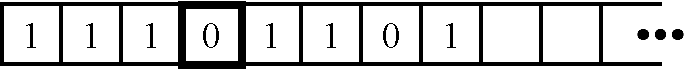
\includegraphics[width=0.5\linewidth]{figures/single-tape-turing-machine.pdf}
    \caption[The tape of a single-tape Turing machine in an arbitrary state.]{The tape of a single-tape Turing machine in an arbitrary state. Note that any multi-tape Turing machines can be efficiently simulated by a single-tape Turing machine~\cite{hartmanis1965computational}, so complexity classes are not affected by changing between single-tape and multi-tape machines.}
    \label{fig:single-tape-turing-machine}
\end{figure}

Everything that can be computed on models of computations we use these days can be computed on a Turing machine~\cite{dershowitz2008natural}.
This hypothesis is known as the Church-Turing thesis.
Related to the Church-Turing thesis is the extended Church-Turing thesis, which states that any physically realizable model of computation can be efficiently simulated on a Turing machine.
That is, can a Turing machine efficiently (in polynomial time) simulate any model of computation?
The quantum computational model brings doubt to this claim.
It is known that quantum computers can efficiently simulate a Turing machine, so they are at least as powerful as classical computers~\cite{bennett1973logical}.
However, there appears to be no efficient algorithm for simulating a quantum computer on a Turing machine.
Furthermore, \textcite{arute2019quantum} experimentally demonstrated a quantum computer sampling from a probability distribution intractable by a classical computer.

\subsection{Complexity Classes}
Complexity classes are sets of computational problems that share some common feature with regard to the computational resources they need to solve some problem~\cite{arora2009computational}.
They are defined in terms of a type of computational problem, computational model, and a bounded resource such as time or space.
In general, most complexity classes describe decision problems solvable by deterministic Turing machines --- though many complexity classes are defined in terms of other types of problems and computational models.
This report mainly focuses on complexity classes involving Turing machines and quantum Turing machines.

The class $\P$ contains all decision problems solvable by a deterministic Turing machine in $O(n^k)$ (polynomial) time for some constant $k$.
Problems that fall under this class are often referred to as tractable or easy problems~\cite{cormen2009introduction}.

\section{Quantum Information}

\section{Quantum Computation}